\subsection{Mechaniken}
Es wurden nun in \textit{Sektion 2} und \textit{Sektion 3} einige Mechaniken und Eigenheiten von älteren und neu erschienen Management Games untersucht und Hypothesen dazu angeführt. Diese Hypothesen und Mechaniken, welche sich als besonders interessant und nutzerfreundlich erweisen, werden nun unter Berücksichtigung der in \textit{Sektion 4.1} erörterten Vorgänge innerhalb einer Bienenkolonie konkretisiert und ausgefeilt. Außerdem werden die in \textit{Sektion 1} definierten Eigenschaften eines Resource Management Games berücksichtigt und versucht, die untersuchten Gegebenheiten (Ressourcen, Ökonomie, Informationsgehalt und Verwaltungsaspekte) möglichst sinnvoll mit den Vorgängen einer Bienenkolonie zu kombinieren, um daraus ein Spiel zu gestalten, welches sehr stark an die echten Vorgänge einer solchen angelehnt ist. Im folgende referenzierte Hypothesen aus \autoref{table:hypotheses} werden mit [HX] abgekürzt, wobei X für die jeweilige Nummer der Hypothese steht.

\subsubsection{Anweisungsstil}
Wie sich in den Interviews und der Analyse von RimWorld gezeigt hat, lassen sich die Art, auf welche Anweisungen an die jeweiligen Einheiten erteilt werden, in \textit{direktes} und \textit{indirektes} Anweisen beziehungsweise Zuweisen. Während in den bereits vorgestellten Titeln meistens auf eine direkte Anweisung der Einheiten zurückgegriffen wird, stellt RimWorld eine Neuerung dar, welche laut [H15] für das Genre des Colony Managements als durchaus positiv von den Probanden aufgefasst wird. Daher wird dieser Anweisungsstil, mitsamt der Prioritätenliste [H13], welche mittels Grafiken verständlicher gemacht wird [H14].

\subsubsection{Ressourcen}
Die im Spiel vorhandenen Ressourcen sind in \autoref{table:resources} aufgelistet. Die Gründe für die Auswahl der Ressourcen sind \textit{Sektion 4.1.1} zu finden. \textit{Honigtau} wird nicht als Ressource implementiert, da diese von lebenden Tieren extrahiert wird, und aufgrund von weiteren benötigten Modellen und Animationen keine weiteren Tiere neben den eigentlichen Bienen implementiert werden. Um das Spiel spannender und etwas komplexer zu gestalten werden verschiedene \textit{Sources}, \textit{Converter} und \textit{Drains} (vgl. \textit{Sektion 1.1.2}) verwendet. Alle involvierten Ressourcen, wie auch baubare Waben, sind in \autoref{image:resourceloop} skizziert. Die Zahlen sind dabei rein experimentell und müssen im Verlauf der Tests gegebenenfalls angepasst werden.

\begin{table}[]
    \centering
    \caption{Verfügbare konkrete Ressourcen}
    \label{table:resources}
    \begin{tabular}{|l|l|}
    \hline
    Nahrung     & Nektar, Honig, Pollen, Royal Jelly, Wasser \\ \hline
    Baumaterial & Bienenwachs                                \\ \hline
    Einheiten   & Königinnen, Drohnen, Arbeitsbienen         \\ \hline
    \end{tabular}
\end{table}



\paragraph{Nektar}
Nektar wird ausschließlich von Blumen extrahiert, welche eine \textit{Source} darstellen. Jedoch ist an jede Blume eine Bedingung geknüpft. Blumen haben ein eigenes Inventar für Nektar und Pollen, welches bei Extraktion durch eine Biene geleert wird und neu regenerieren muss. Eine Biene sollte also frequentiv die Blumen wechseln, um möglichst viele Ressourcen zu sammeln. Nektar hat eine gewisse Lebensdauer und wird nach einiger Zeit schlecht, wodurch eine gewisse Anzahl von Nektar aus dem Spiel entfernt wird. Diese Lebensdauer agiert dadurch als \textit{Drain}.

\paragraph{Pollen}
Die zweite Ressource sind die Pollen, welche ebenfalls von Blumen extrahiert werden. Pollen können unter anderem verwendet werden, um neue Blumen zu pflanzen und spielen daher gerade im Frühling eine große Rolle, aber auch für das Herstellen für Bienenwachs und Gelée Royal. Pollen besitzen eine etwas längere Lebensdauer und können daher über den Winter gelagert werden. Dadurch, dass Pollen mehrere Anwendungsfälle besitzen, muss der Spieler abwägen, für welchen er diese Ressource am ehesten verwendet beziehungsweise wie er die vorhandenen Ressourcen aufteilt.

\paragraph{Honig}
Honig ist eine manuell hergestellte Ressource, welche an einem \textit{Evaporator}, also einer leicht umgebauten Wabe, von einer Biene hergestellt werden kann. Dieser Evaporator stellt, neben den anderen baubaren Waben, einen \textit{Converter} dar. Ein wichtiger Aspekt des Honigs ist der Fakt, dass man mehr als ein Nektar pro Honig verwenden muss, damit der Spieler abwägen muss, ob es die Herstellung wert ist. Dadurch entsteht mehr Komplexität und der Spieler besitzt Entscheidungsfreiheit. So könnten manche Spieler versuchen, lediglich genug Honig für den Winter herzustellen, und andere wiederum jeglichen Nektar direkt in Honig umwandeln. Es entsteht somit eine mögliche \textit{Strategie}.

\paragraph{Bienenwachs}
Entgegen der anderen Ressourcen ist Bienenwachs keine Nahrung. Diese Ressource wird einzig und allein für den Bau neuer Strukturen verwendet. Diese Strukturen werden im Folgenden näher erläutert. Bienenwachs muss an einem \textit{Mixer} hergestellt werden, welcher sowohl Honig als auch Pollen verwendet, um neues Bienenwachs herzustellen. Aus diesem Bienenwachs können dann \textit{Brutwaben, Lagerwaben} und \textit{Refiner} hergestellt werden, wie auch ein neuer Stock, sollte man den gegebenen verlagern wollen.

\paragraph{Gelée Royal}
Eine weitere fundamentale Ressource ist das Gelée Royal oder auch \textit{Royal Jelly}, welches an einem \textit{Refiner} durch Vermischen von Pollen und Honig erzeugt werden kann. Diese Ressource ist wichtig für das Heranziehen einer neuen Königin und wird in die Brutwabe einer \textit{Arbeitsbienenlarve} gegeben, damit diese sich zu einer Königin entwickelt.

\paragraph{Wasser}
Die einzige nicht vom Spieler sammelbare oder lagerbare Ressource ist Wasser. Dieses müssen die Bienen durch Nahrung aufnehmen (Nektar besitzt mehr Wasser als Honig), oder über das Trinken an einem Fluss. Da im Winter keine Ausflüge gestattet sind, ist es wichtig, dass Bienen vor dem Winter genug Wasser zu sich nehmen, um nicht zu verdursten.

\paragraph{Königin, Drohne und Arbeitsbiene}
Diese greifbaren Ressourcen sind das Fundament des Spiels, wobei neue Bienen, analog zu \textit{Sektion 4.1.3}, Kasten-spezifisch herangezogen werden können, mehr dazu im folgenden Abschnitt.

\begin{figure}
    \begin{center}
        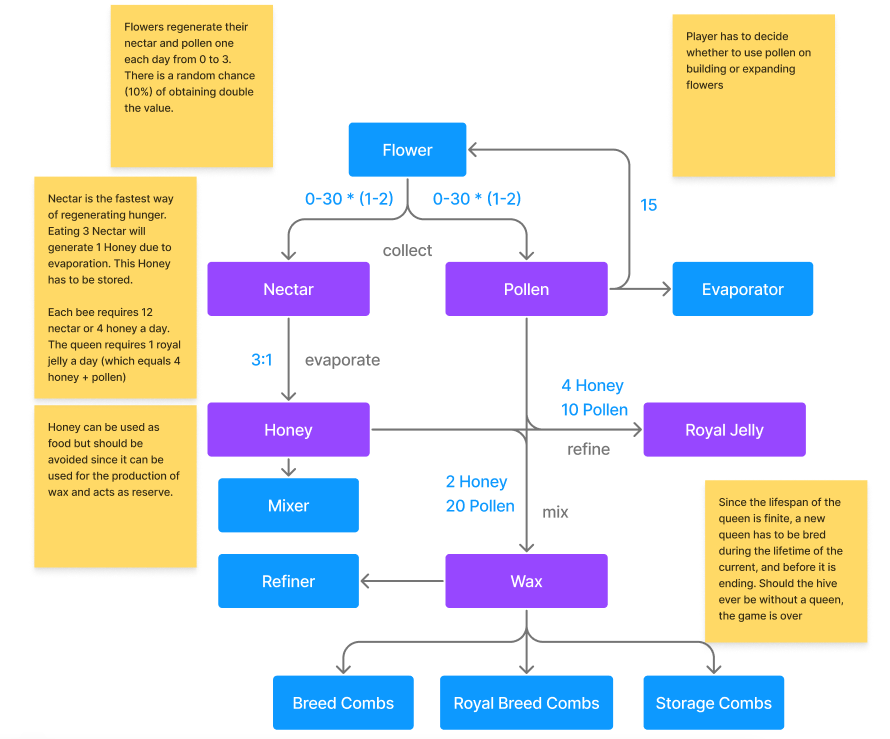
\includegraphics[width=300px]{0.bilder/resourceloop.png}
    \end{center}
    \caption{Ressourcenverlauf und mögliche Umwandlungen} \label{image:resourceloop}
\end{figure}

\subsubsection{Jahreszeiten}
Es gibt vier verschiedene Jahreszeiten, \textit{Frühling, Sommer, Herbst} und \textit{Winter}. Alle 30 Tage wechselt die Jahreszeit zur jeweils nächsten. Jede Jahreszeit ist dabei anders und bietet andere, mögliche Events. Jegliche Angaben von Chancen sind dabei rein experimentell und müssen im späteren Verlauf getestet werden.

\paragraph{Frühling} ist die Zeit, in welcher neue Blumen sprießen. Es gibt ein besonderes Event namens \textit{Pollenflug}, wobei besonders viele Blumen sprießen, was es dem Spieler durchaus erleichtern kann, neue Nahrung zu beschaffen. Das Event hat eine Chance von $\frac{1}{30}$ pro Tag zu passieren, und kann pro Jahr maximal ein Mal geschehen.

\paragraph{Sommer} ist die Zeit der Hitze und des \textit{Schwärmens}. Deshalb gibt es zwei Events welche passieren können, das erste ist die \textit{Dürre}, wobei einige Blumen sterben und manche Flüsse austrocknen. Die Chance dafür ist pro Tag $\frac{1}{60}$. Das zweite ist das Schwärmen, welches jedes Jahr erneut passiert, insofern eine Königin vorhanden ist. Dabei wird angegeben, dass die Königin den Stock verlassen wird. Deshalb ist der Spieler dazu gezwungen, eine neue Königin heranzuziehen, da ansonsten keine Königin mehr vorhanden sein wird. Die Königin wird dabei einen kleinen Anteil der Kolonie mitnehmen (mindestens eine \textit{Arbeitsbiene} und \textit{20\%} der Arbeitsbienen). Diese Zahl ist variabel und wird gegebenenfalls angepasst. Der Spieler wird also etwas zurückgesetzt und gezwungen, zu handeln, was die Herausforderung durchaus erschwert. 

\paragraph{Herbst} bringt zwei negative Events mit sich. Es kann jeden Tag mit einer $\frac{1}{60}$ Chance passieren, dass jegliche Blumen weniger Ertrag geben in entweder Pollen oder Nektar. Auch hier wird der Spieler dazu gezwungen, sich anzupassen und sinnvoll darauf zu reagieren. Zudem ist die Chance auf Regen durchaus etwas höher, als sonst in den Jahreszeiten. Als wiederkehrendes Event, analog zum Schwärmen, steht jedes Jahr der \textit{Drohnenkrieg} beziehungsweise die \textit{Drohnenschlacht} an, wobei sämtliche Drohnen aus dem Stock 

\paragraph{Winter} ist die Zeit des Notstands. Die Bienen sind in dieser Zeit nicht ausflugfähig und müssen in ihrem Bienenstock warten, bis der Winter endet. Daher muss darauf geachtet werden, dass genug Honig gelagert ist, damit die Kolonie überleben kann. Sollte Regen während dieser Zeit fallen, ist dieser stattdessen Schnee. Es sterben zu dieser Jahreszeit sämtliche Blumen ab, wodurch, selbst wenn eine Biene rausfliegen würde, es keine Möglichkeit gibt, Nahrung zu beschaffen.


\begin{figure}
    \begin{center}
        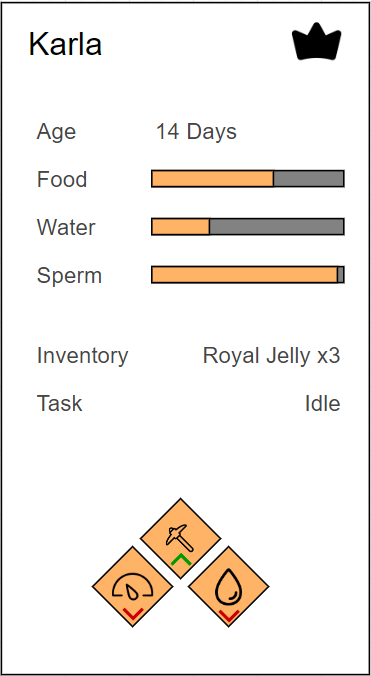
\includegraphics[width=100px]{0.bilder/beeinfodraw.PNG}
    \end{center}
    \caption{Skizze des Informationsfensters einer ausgewählten Biene} \label{image:beeinfodraw}
\end{figure}

\subsubsection{Bienen}
Die Bienen sind das Herzstück des Spiels und werden analog zu \textit{RimWorld} indirekt gesteuert. Eine Biene hat mehrere Eigenschaften. Sämtliche aufgelisteten Eigenschaften sind visuell dargestellt als Skizze in \autoref{image:beeinfodraw}.

\paragraph{Kasten}
Es gibt analog zu einer realen Bienenkolonie drei verschiedene Kasten. Jede Biene besitzt eine Variable in Form einer Enum, welche angibt, ob es sich um eine Königin, eine Drohne oder eine Arbeitsbiene handelt. Aufgrund dieser Information werden etliche Entscheidungen getroffen, darunter das gezeigte Modell, wovon es drei verschiedene für jede Kaste gibt, die möglichen ausführbaren Aktionen und die Lebensdauer. Es können kastenspezifisch neue Bienen herangezogen werden. Wie auch in der realen Welt werden für die Arbeitsbienen befruchtete Eier benötigt, für die Königinnen befruchtete Eier und Royal Jelly, und für die Drohnen lediglich unbefruchtete Eier. Diese Mechanik ist in \autoref{image:reproductionloop} schematisch dargestellt.

\begin{figure}
    \begin{center}
        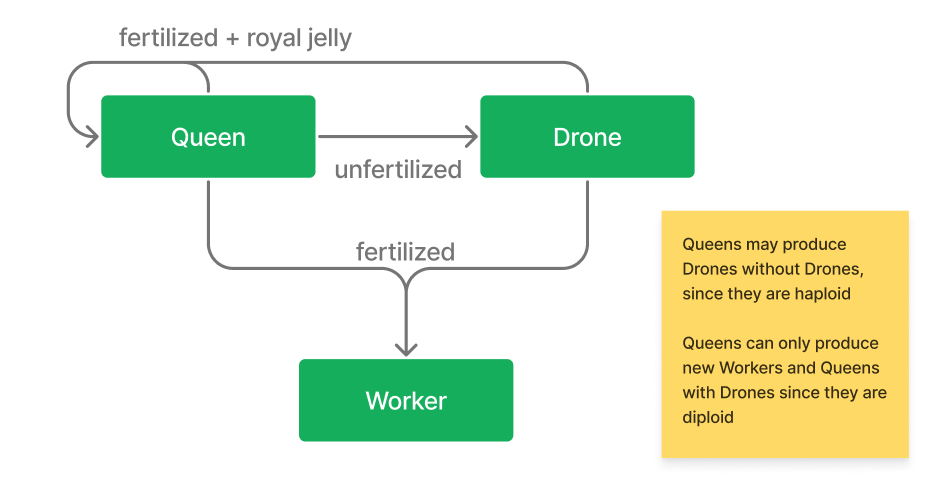
\includegraphics[width=300px]{0.bilder/reproductionloop.png}
    \end{center}
    \caption{Reproduktionsverhalten der Bienen} \label{image:reproductionloop}
\end{figure}

\paragraph{Alter} 
Das Alter der Biene ist von zentraler Bedeutung. Für die Königin ist es entscheidend einzuschätzen, wie lange diese noch lebt, für die Arbeitsbienen ist es wichtig zu erkennen, welche Arbeiten und Aufgaben diese übernehmen kann. Eine Biene am Ende ihres Lebens ist biologisch nicht mehr in der Lage, die neue Brut zu füttern, und dient lediglich dem Sammeln von Ressourcen.

\paragraph{Hunger} 
Eine Biene hat das Bedürfnis nach Nahrung. Der Nahrungsbalken wird mit der Zeit weniger, weshalb die Biene Nahrung beschaffen muss, jedoch nicht aktiv. Ist Nahrung vorhanden und die Biene erreicht einen Schwellenwert, wird sich diese Biene die Nahrung eigenständig aus dem Lager entnehmen. Ist der Wert der Nahrung zu lange auf 0, stirbt die Biene. Die voreingestellte Reihenfolge der verspeisten Nahrung lautet:

\begin{center}
    Nektar > Honig > Pollen
\end{center} Royal Jelly wird nicht von den Arbeitern angerührt und wird lediglich von der Königin verspeist, genau so wie für das Heranziehen neuer Königinnen zur Larve gegeben. Stetige Bewegung sorgt für schnelleren Hunger. Die Reihenfolge der Nahrung kann vom Spieler angepasst werden, wodurch mehr Entscheidungsfreiheit gegeben ist und mehr Taktik angewandt werden kann. So könnte ein Spieler möglichst viele Pollen sammeln und diese als primäre Nahrungsquelle nutzen. Natürlich müssen diese Mechaniken ausgiebig getestet werden, sodass verschiedene Strategien nicht zu unausgeglichen sind.

\paragraph{Durst} 
Bienen benötigen Flüssigkeit, genauer gesagt Wasser. Dieses wird nicht im Stock gelagert, sondern an Flüssen getrunken. Je mehr sich eine Biene bewegt, desto mehr Flüssigkeit benötigt diese. Sinkt dieser Wert auf 0, wird die Biene nach kurzer Zeit sterben.

\paragraph{Samen} 
Diese Eigenschaft hat lediglich eine Königin, und gibt an, wie viel Samen der Drohnen noch vorhanden sind um neue und befruchtete Eier zu legen. Es ist wichtig darauf ein Auge zu haben, da ohne verfügbare Samen weder Arbeitsbienen, noch Königinnen herangezogen werden können.

\paragraph{Inventar} 
Das Inventar besitzt jede Biene und zeigt an, was diese gerade trägt. Getragen werden können Nektar, Pollen, Honig, Royal Jelly und Bienenwachs. Es kann zeitgleich nur eine Art von etwas getragen werden, und die Menge richtet sich nach der Art des Getragenen. Die Ausnahme dabei stellen Pollen dar, welche in den \textit{Pollensäckchen} zeitgleich zu anderen Dingen getragen werden.

\paragraph{Auftrag} 
Der momentane Auftrag ist ebenfalls Teil der Biene. Dieser zeigt dem Nutzer, was diese Biene gerade vorhat und wieso sie sich zu der bestimmten Stelle bewegt.

\paragraph{Genetische Eigenschaften / Traits} 
Die genetischen Eigenschaften beziehungsweise \textit{Traits} sind immer exakt drei Stück und werden nach [H6] in überschaubarer Anzahl gehalten und so benannt, dass aus dem Namen der Effekt grundlegend ersichtlich ist. Diese können sowohl \textit{positive} als auch \textit{negative} Auswirkungen auf die Effizienz der einzelnen Biene haben, wobei nicht eindeutig erkennbar sein soll, welcher der effektiv beste oder schlechteste Trait ist, der zur Auswahl steht, um [H7] nachzugehen, und Nutzer-eigene Strategien zu fördern. Die möglichen Traits und ihre Wahrscheinlichkeiten sind in \autoref{table:traits} zu finden. Die Traits sind vererbbar, wobei bei der Vererbung eine Chance besteht, dass ein Trait \textit{mutiert} und deshalb in einen anderen, zufälligen, geändert wird. Wird eine Königin von mehreren verschiedenen Drohnen besamt, werden die Erbinformationen gespeichert. Ob der jeweilige Trait nun von der Seite des Vaters oder der Seite der Mutter übernommen wird, ist gleichverteilt 50:50. Seien die besamenden Drohnen folgende:

\begin{itemize}
    \item Drohne A: Schillernd, Arbeitsfreudig, Gesegnet
    \item Drohne B: Schillernd, Arbeitsfreudig, Verflucht
    \item Drohne C: Schillernd, Großer Magen, Verdampfer
\end{itemize} Und die Königin besäße folgende Eigenschaften:

\begin{itemize}
    \item Königin: Schillernd, Großer Magen, Empfänglich
\end{itemize} Dann gelten folgende Chancen für die Traits der Brut:

\begin{itemize}
    \item Schillernd: $100\%$
    \item Empfänglich: $\frac{1}{2}$
    \item Großer Magen: $\frac{1}{3} + \frac{1}{2} = \frac{5}{6}$
    \item Arbeitsfreudig: $\frac{2}{3} \times \frac{1}{2} = \frac{1}{3}$
    \item Gesegnet: $\frac{1}{3} \times \frac{1}{2} = \frac{1}{6}$
    \item Verflucht: $\frac{1}{3} \times \frac{1}{2} = \frac{1}{6}$
    \item Verdampfer: $\frac{1}{3} \times \frac{1}{2} = \frac{1}{6}$
\end{itemize} Die Traits, welche speziell auf eine gewisse Art von Kaste gelten, werden im Hintergrund gespeichert und es wird ein neuer Trait gezogen. Dieser wird sich vorgemerkt. Sollte die Arbeitsbienenlarve also zur Königin herangezogen werden, wird der vorgemerkte Trait durch den Erstgezogenen ersetzt.

\paragraph{Mutation}
Damit eine Diversität entstehen kann, und nicht stetig die gleichen Traits in der Kolonie weitervererbt werden, bedarf es der Möglichkeit einer Mutation. Es besteht eine geringe Chance, dass \textit{nach dem Ziehen} eines vererbten Traits, dieser Trait durch einen völlig anderen ersetzt wird.
% Please add the following required packages to your document preamble:
% \usepackage{graphicx}
\begin{table}[]
    \centering
    \caption{Mögliche Traits einer Biene}
    \label{table:traits}
    \resizebox{\columnwidth}{!}{%
    \begin{tabular}{|l|l|l|}
    \hline
    Arbeitsfreudig / Arbeitsscheu (Alle)        & Erledigt alle Aufgaben 10\% schneller / langsamer                                        & 12\% \\ \hline
    Sammelfreudig / Sammelscheu (Arbeitsbiene)  & Sammelt Ressourcen 15\% schneller / langsamer                                            & 12\% \\ \hline
    Fingerfertig / Grobmotorisch (Arbeitsbiene) & Stellt neue Ressourcen 10\% schneller / langsamer her.                                   & 12\% \\ \hline
    Sparsam / Freigiebig (Arbeitsbiene)         & Verbraucht beim Füttern etwas weniger / mehr Nahrung.                                    & 12\% \\ \hline
    Empfänglich / Unempfänglich (Königin)       & Benötigt weniger / mehr Drohnen um die Samen zu füllen und hat mehr / weniger Kapazität. & 12\% \\ \hline
    Gesegnet / Verflucht (Alle)                 & Lebt ein längeres / kürzeres Leben.                                                      & 12\% \\ \hline
    Wasserspeicher / Verdampfer (Alle)          & Benötigt weniger / mehr Wasser und verbraucht weniger / mehr.                            & 12\% \\ \hline
    Kleiner / Großer Magen (Alle)               & Benötigt weniger / mehr Nahrung und verbraucht weniger / mehr.                           & 12\% \\ \hline
    Königliche Immunität (Drone)                & Die Drohne ist ausgenommen von der Drohnenschlacht.                                      & 2\%  \\ \hline
    Schillernd (Alle)                           & Die Biene sieht anders aus als gewöhnliche Bienen.                                       & 2\%  \\ \hline
    \end{tabular}%
    }
    \end{table}



\subsubsection{Aktionen}
Es gibt 6 verschiedene, vom Spieler ausführbare, Anordnungen. Diese werden verwendet, um die Bienen indirekt zu steuern und den Stock somit möglichst am Leben zu erhalten.

\paragraph{Sammeln} wird verwendet, um von den in der Spielwelt vorhandenen Blumen den Nektar und die Pollen zu extrahieren. Diese Aktion ist lediglich von Arbeitsbienen im späten Alter ausführbar.

\paragraph{Bestäuben} verwendet Pollen, um neue Blumen zu erstellen, welche als weitere Quelle von Nektar und Pollen agieren. Dies kann sinnvoll sein, sollten nicht genug Blumen vorhanden sein, etwa im Frühling nach einem harten Winter. Diese Aktion ist ebenfalls nur von älteren Bienen ausführbar.

\paragraph{Besamen} ist eine Aktion, welche lediglich den Drohnen vorbehalten ist. Mit Auswahl der Königin finden sich nacheinander Drohnen, bis die Königin keine weiteren Samen speichern kann.

\paragraph{Eier legen} wird lediglich von der Königin ausgeführt. Nach Auswahl einer passenden Brutwabe (normale Brutwabe oder königliche Brutwabe), fliegt die Königin zu der jeweiligen Stelle und legt ein Ei ab. Ob dieses befruchtet ist oder nicht hängt davon ab, ob die Königin Samen gespeichert hat.

\paragraph{Abbrechen} wird verwendet, um eine bereits ausgeführte Anordnung zurückzuziehen. Anders als die anderen Aktionen ist hierfür keine Biene nötig.

\paragraph{Zerstören} kann verwendet werden, um vom Spieler gebaute Strukturen wieder zu vernichten. Diese Aktion ist lediglich von mittelalten Arbeitsbienen ausführbar und ist auf den Bienenstock beschränkt.

\subsubsection{Strukturen}
Es gibt, analog zu den Aktionen, 6 verschiedene, baubare Strukturen. Diese dienen in den meisten Fällen als \textit{Converter} und Arbeitsstätte der Bienen, aber auch als Lagerplatz. Sämtliche baubare Strukturen sind \autoref{image:resourceloop} zu entnehmen.

\paragraph{Evaporator} ist ein Converter, um aus Nektar Honig herzustellen, und dient der Erfüllung von [H12]. Dieser wird, wie in \autoref{image:resourceloop} erkennbar, aus Pollen hergestellt. Mit Klick auf den gebauten Evaporator können Aufträge erstellt werden, wodurch festgelegt werden kann, wie viel Honig hergestellt werden soll. Für diese Aufträge müssen Bienen am Evaporator arbeiten.

\paragraph{Mixer} ist ebenfalls ein Converter, erfüllt ebenfalls [H12] und wird verwendet, um aus Honig und Pollen Bienenwachs herzustellen. Zum Bau dieser Struktur wird Honig verwendet, wodurch ein zuvor gebauter Evaporator sinnvoll ist. Das Auftragssystem ist analog zum Evaporator.

\paragraph{Refiner} wird verwendet, um aus Honig und Pollen Royal Jelly herzustellen, wobei für den Bau dieser Struktur Bienenwachs verwendet wird. Dadurch kann es sinnvoll sein, einen Mixer gebaut zu haben. Das Auftragssystem ist analog zu dem Evaporator und dem Mixer und dient ebenfalls der Erfüllung von [H12].

\paragraph{Lagerwaben} sind essenziell zum Speichern und Lagern bestimmter Ressourcen. In diesen Lagerwaben können Nektar, Pollen, Honig, Royal Jelly und Bienenwachs gespeichert werden, wobei eine Lagerwabe nur eine Art von Ressource halten kann, und ebenfalls ein quantitatives Limit für diese Ressource besitzt. Für den Bau einer Lagerwabe wird Bienenwachs verwendet. Diese Lagerstruktur dient als klare, baubare Struktur der Erfüllung von [H9].

\paragraph{Brutwaben} werden für die Fortpflanzung beziehungsweise Eierhaltung der Königin verwendet. Junge Arbeitsbienen werden lediglich angeordnet Nektar oder Honig zu liefern. Wird die Larve zu einer Puppe, muss außerdem von einer Arbeitsbiene die Brutwabe durch Bienenwachs bedeckt werden.

\paragraph{Königliche Brutwaben} sind ähnlich zu den normalen Brutwaben, mit der Ausnahme, dass lediglich befruchtete Eier dort gelegt werden können, und die jungen Arbeitsbienen zu der Larve Royal Jelly geben, falls vorhanden.

\subsubsection{Brutvorgang}
Um neue Bienen herzustellen werden, wie bereits zuvor erläutert und in \autoref{image:reproductionloop} erkennbar, verschiedene Bienen für verschiedene Resultate benötigt. Wird ein Ei in eine Brutkammer gelegt, beginnt ab diesem Zeitpunkt die Metamorphose, analog zu den In \textit{Sektion 4.1.4} erläuterten Vorgängen. Das gelegte Ei wird nach einer gegebenen Zeit zu einer Larve, danach zu einer Puppe und anschließend zu einer voll ausgewachsenen Biene.

\paragraph{Stadium 1: Ei} Das Ei liegt nach dem Legen in der Brutwabe. Zu diesem Stadium ist lediglich erkennbar, ob befruchtet oder unbefruchtet. Die Wabe muss ein Mal mit Nahrung, vorzugsweise Nektar oder Honig, gefüllt werden, damit das Ei überlebt. Nach einigen Tagen schlüpft daraus eine Larve und die Nahrung in der Brutwabe ist verbraucht.

\paragraph{Stadium 2: Larve} Die Larve ist das Stadium, in welchem Royal Jelly dazugegeben werden kann. Liegt das Ei in einer Königlichen Brutkammer, wird einmalig Royal Jelly statt gewöhnlicher Nahrung dazugegeben. Damit entwickelt sich eine königliche Puppe statt einer herkömmlichen und die Nahrung wird verbraucht.

\paragraph{Stadium 3: Puppe} Die Puppe benötigt, anders als die anderen Stadien, zusätzlich zur Nahrung noch Bienenwachs, welches die Brutwabe bedeckt. Zuerst muss Nahrung dazugegeben, danach die Wabe bedeckt werden. Sobald die Biene alt genug ist, schlüpft sie aus der Puppe und bricht durch die Wachsschicht. Eine erwachsene Biene ist somit herangereift.

\paragraph{Stadium 4: Ausgewachsen} Das ausgewachsene Stadium ermöglicht sämtliche Aktionen einer Biene. In diesem Stadium befinden sich die meisten Bienen. 

\begin{figure}
    \begin{center}
        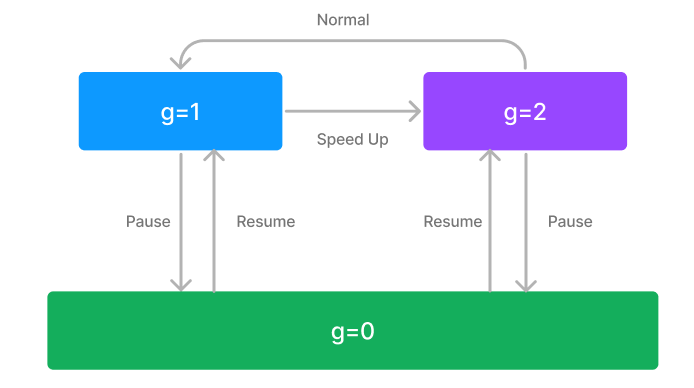
\includegraphics[width=300px]{0.bilder/timecontrol.png}
    \end{center}
    \caption{Zeitsteuerung Zustandsdiagramm} \label{image:timecontrol}
\end{figure}

\subsubsection{Zeitsteuerung}
Analog zu RimWorld wird nach [H21] eine Zeitsteuerung zur besseren Kontrolle eingeführt. Zur Auswahl stehen dabei \textit{Pause} beziehungsweise \textit{Fortführen} (engl. \textit{Resume}) als sich abwechselnde Zustände, und weiterhin \textit{Normal} und \textit{Erhöht}, wobei \textit{Pause} die Geschwindigkeit des Spiels auf $g=0$ setzt, \textit{Normal} die Geschwindigkeit auf $g=1$ setzt, und \textit{Erhöht} die Geschwindigkeit auf $g=2$ setzt. Allerdings wird eine intelligentere Logik verwendet, um das Nutzererlebnis zu erhöhen, welche in \autoref{image:timecontrol} veranschaulicht wird. Pausiert der Nutzer das Spiel, während die Geschwindigkeit auf g=2 steht, wird sich dieser Wert gemerkt, und bei Klick auf den nun vorhandenen Resume-Button wiederhergestellt. Analog funktioniert dieser Prozess auch bei g=1.

